\section{Related Work}
\subsection{Convolutional Neural Networks}

Convolutional Neural Networks (CNNs) have become a standard approach for image segmentation tasks. This section discusses three important CNN architectures for segmentation: FCN, UNet++ and DeepLabV3+, providing a mathematical overview based on the foundational principles and improvements proposed in their respective works.

\subsubsection{Fully Convolutional Networks (FCN)}

The Fully Convolutional Network (FCN) \cite{long2015fcn} was one of the pioneering architectures for dense predictions in semantic segmentation. Unlike traditional CNNs, FCNs replace fully connected layers with convolutional layers, enabling the model to predict a segmentation mask with spatial dimensions corresponding to the input image. The core idea is to use convolutional and pooling layers to produce feature maps at various scales, followed by a deconvolution (upsampling) layer to restore the original image resolution.

The output of an FCN can be expressed as:
\[
\hat{y} = f(W \ast X + b)
\]
where $W$ represents the learned convolutional weights, $X$ is the input image, $b$ is the bias term, and $f$ is the activation function. Using convolutional layers throughout ensures the model can handle inputs of arbitrary sizes, and the final upsampling layer reconstructs the pixel-wise segmentation map.

\subsubsection{UNet++}

UNet++ \cite{zhou2019unet++} improves upon the original U-Net architecture by introducing nested and dense skip connections between the encoder and decoder paths, bridging the semantic gap between feature maps at different scales. This refinement reduces the complexity of the decoder and improves the network's ability to capture fine-grained details, particularly in medical imaging tasks.

The main innovation in UNet++ is the re-designed skip connections:
\[
F_{i,j} = H_{i,j} \left( F_{i-1,j} + \sum_{k=0}^{j-1} H_{i,k} \right)
\]
where $F_{i,j}$ represents the feature map at the $i$-th depth and $j$-th layer, and $H_{i,j}$ denotes the convolutional operations. The nested architecture allows for the gradual refinement of feature maps at each level, making it more effective in learning from complex and hierarchical data.

\subsubsection{DeepLabV3+}

DeepLabV3+ \cite{chen2018deeplabv3+} builds on DeepLabV3 by integrating an encoder-decoder structure and employing atrous (dilated) convolutions to capture multi-scale context efficiently. Atrous convolution introduces the dilation rate, $r$, which controls the spacing between kernel elements. This allows the network to expand the receptive field without increasing the number of parameters.

The atrous convolution operation is defined as:
\[
y[i] = \sum_k x[i + r \cdot k] \cdot w[k]
\]
where $x$ is the input, $w$ represents the filter weights, and $r$ is the dilation rate. DeepLabV3+ also includes an Atrous Spatial Pyramid Pooling (ASPP) module that applies multiple atrous convolutions with different rates, allowing the model to capture information at multiple scales. The decoder then upsamples the feature maps to generate the final segmentation mask.

\subsection{Graph Neural Networks: Graph-FCN and CNN-G}

Deep learning has made significant advancements in semantic segmentation by classifying pixels in images. However, during high-level feature extraction, it often ignores the local spatial information, which is important for accurate segmentation. Graph-based models address this limitation by including the missing local context.

\subsubsection{Graph-FCN}

Graph-FCN combines graph convolutional networks (GCNs) with fully convolutional networks (FCNs) to capture local spatial relationships in images. Initially, a convolutional network converts the image grid data into a graph structure, transforming the semantic segmentation task into a graph node classification problem. The graph convolutional network is then applied to classify the nodes in this graph, effectively solving the segmentation challenge.

FCN-16s generates feature maps, and node annotations are initialized by combining upsampled feature vectors and node locations. Labels for nodes are obtained by pooling the raw label image during training. The process is shown in Figure~\ref{fig:graphfcn_node_init}.

\begin{figure}
    \centering
    % \fbox{\rule{0pt}{2in} \rule{0.9\linewidth}{0pt}}
    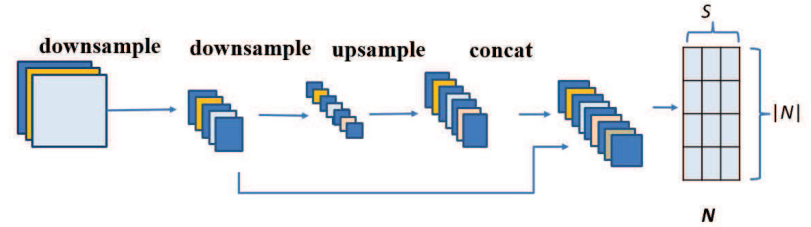
\includegraphics[width=0.8\linewidth]{images/graphfcn_node_init.png}
    \caption{Graph-FCN node initialization. From ~\cite{lu2020graphfcnimagesemanticsegmentation}.}
    \label{fig:graphfcn_node_init}
\end{figure}

In the graph model, edges are represented by an adjacency matrix, where each node is connected to its nearest $l$ nodes. These connections allow node annotations to transfer through the edges in the graph neural network.

FCN-16s handles node classification and graph model initialization on a small feature map, while a 2-layer GCN classifies the nodes within the graph. Cross-entropy loss is computed for both outputs, and like FCN-16s, Graph-FCN is trained end-to-end. The output of the prediction process is the output of the convolutional network. The graph model is only used during the training.

The structure of the Graph-FCN model is shown in Figure~\ref{fig:graphfcn_structure}.
\begin{figure}
    \centering
    % \fbox{\rule{0pt}{2in} \rule{0.9\linewidth}{0pt}}
    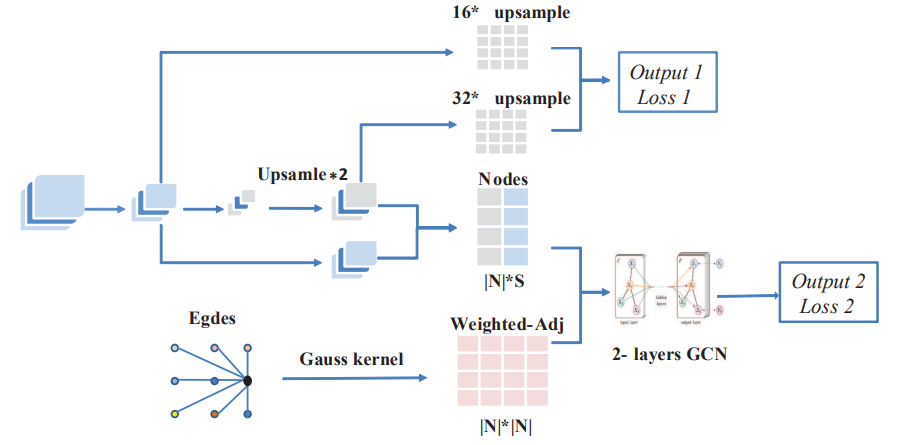
\includegraphics[width=0.8\linewidth]{images/graphfcn_structure.png}
    \caption{Graph-FCN model structure. From ~\cite{lu2020graphfcnimagesemanticsegmentation}.}
    \label{fig:graphfcn_structure}
\end{figure}

\subsubsection{CNN-G}

CNN-G builds on the Graph-FCN model by incorporating a graph-based approach with a convolutional neural network. Two types of structure models are used in CNN-G: distance-based and semantic-based, solved by GCN and GAT, respectively. The distance-based model captures the spatial relationships between nodes, while the semantic-based model focuses on the semantic relationships.

Using a graph attention network (GAT) enables flexible feature extraction across various receptive fields. This approach allows the model to integrate both structure learning and feature extraction.

\textbf{Distance-Based Structure:} Based on the assumption that the closer nodes are more correlated, the Gauss kernel function is used to generate the weighted edges.

The adjacent matrix $A = [e_{ij}]_{|N| \times |N|}$ is used to represent the edge set:

\[
e_{ij} = \begin{cases} \exp \left( -\frac{\|p_i - p_j\|^2}{\sigma^2} \right), & \text{an edge between } n_i \text{ and } n_j \\ 0, & \text{otherwise} \end{cases}.
\]

To simplify the calculation, we make the nodes connect to the $l$ closest nodes.

\textbf{Semantic-based model:} The initial attention coefficient $c_{ij}$ is used to measure the correlation between two nodes. The features of nodes with the same category will be more similar, the attention coefficient between each other will be larger, and the similarity is gradually strengthened in the iteration. A linear transformation is taken to map the concatenation of two nodes' features into a real number: 
\[
c_{ij} = a \left( n_i' || n_j' \right)
\]
The final attention coefficient is obtained through the normalization of all neighborhood nodes: 
\[
e_{ij} = \frac{\exp(c_{ij})}{\sum_{k \in neib_{i}} \exp(c_{ik})}.
\]
When the graph structure is unknown, the matrix $A_{\text{att}} = [e_{ij}]_{|N| \times |N|}$ can be taken as the adjacency matrix. In this case, the edge set is generated by the calculation of the attention coefficients.

In each case, the model generates two outputs, $y1$ and $y2$, which corresponds to two losses, $loss1$ and $loss2$. Both share the convolutional layer's extracted features. The final prediction is based on $y1$. Similar to Graph-FCN, the graph model is only used during training.

The structure of the CNN-G model is shown in Figure~\ref{fig:cnng_structure}.
\begin{figure}
    \centering
    % \fbox{\rule{0pt}{2in} \rule{0.9\linewidth}{0pt}}
    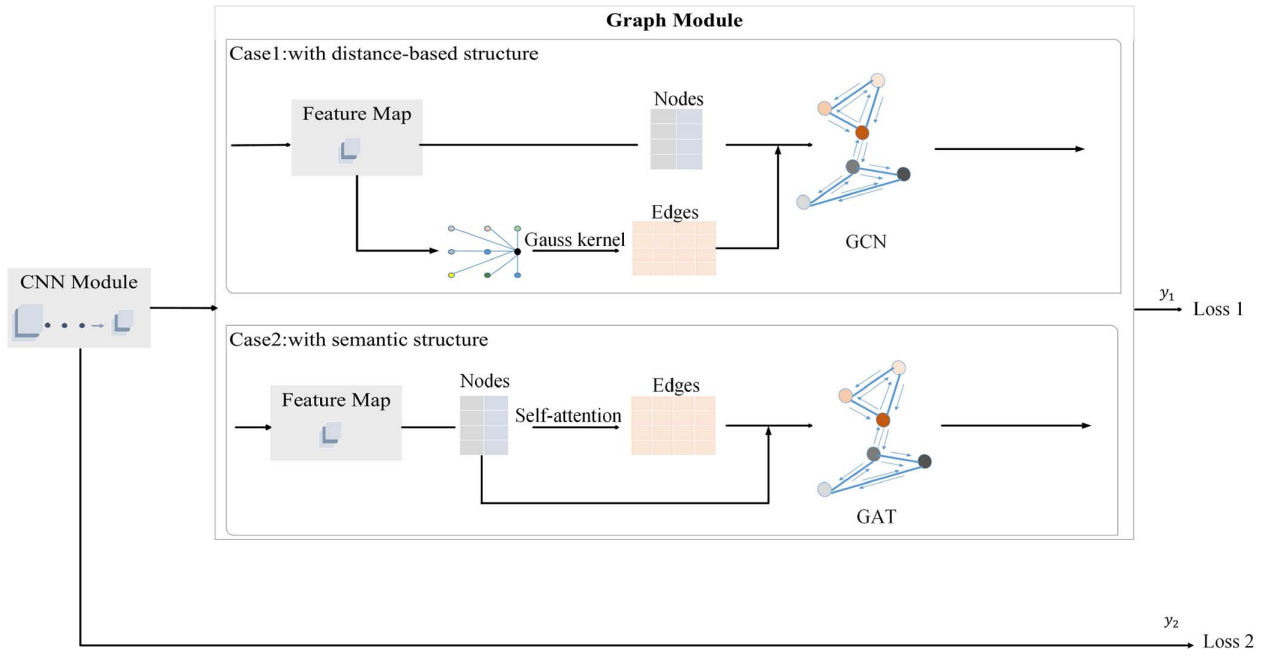
\includegraphics[width=0.8\linewidth]{images/cnng_structure.png}
    \caption{CNN-G model structure. From ~\cite{9103557}.}
    \label{fig:cnng_structure}
\end{figure}

\subsection{Transformer based approaches}
\subsubsection{TransUnet}
TransUNet \cite{chen2021transunettransformersmakestrong} has emerged as a robust framework for medical image segmentation by combining the strengths of U-Net and Transformer architectures.

TransUNet addresses these limitations by introducing a hybrid architecture that leverages both CNNs and Transformers. The encoder consists of a CNN followed by a Transformer module. The CNN is used to extract feature maps from the input images, which are then tokenized into image patches and fed into the Transformer. This CNN-Transformer hybrid allows TransUNet to capture detailed spatial features (via CNN) and global context (via the Transformer) simultaneously.

In the decoder, a cascaded upsampling module (CUP) is employed, consisting of multiple upsampling blocks with convolutional layers and ReLU activation. These upsampled features are combined with the high-resolution CNN feature maps from the encoder through skip connections, similar to the U-Net structure, enabling precise localization. This U-Net-like design ensures that TransUNet can recover lost spatial detail while preserving the high-level semantic understanding captured by the Transformer.

\subsubsection{Seg Former}
SegFormer \cite{xie2021segformersimpleefficientdesign} framework consists of two main modules: A hierarchical Transformer
encoder to extract coarse and fine features; and a lightweight All-MLP decoder to directly fuse these multi-level features and predict the semantic segmentation mask.
\begin{itemize}
    \item \textbf{Hierarchial Transformer Encoder}: designed to generate multi-scale features by progressively reducing the spatial resolution through a series of Mix Transformer (MiT) blocks. This encoder eliminates the need for positional encodings, making it adaptable to varying image sizes. Each MiT block employs overlapping patch embeddings and an efficient self-attention mechanism that reduces computational complexity, allowing it to handle high-resolution inputs. By producing features at multiple resolutions—{1/4, 1/8, 1/16, and 1/32} of the original size—it captures both local and global contexts for improved segmentation of complex objects. 
    \item \textbf{Lightweight All-MLP decoder}: It consists solely of MLP layers, which reduces computational overhead. The decoder first unifies the channel dimensions of the multi-level features, upsampling them to a common resolution before concatenation. This process enables the decoder to leverage fine-grained details and contextual information, ultimately generating a precise semantic segmentation mask. The lightweight design of the MLP decoder ensures high accuracy while maintaining low latency, making SegFormer suitable for real-time applications.
\end{itemize}

\subsubsection{Mask Former}
Mask Former \cite{cheng2021perpixelclassificationneedsemantic} architecture consists of three main components:
\begin{itemize}
    \item \textbf{Pixel-Level Module}: The pixel-level module extracts per-pixel embeddings from the image features. A backbone network (e.g., ResNet or Swin Transformer) first processes the input image to obtain low-resolution feature maps. These feature maps are then gradually upsampled using a lightweight pixel decoder based on the Feature Pyramid Network (FPN) to produce high-resolution, per-pixel embeddings.
    \item \textbf{Transformer Module}: The transformer module uses a standard decoder with learnable queries to compute global embeddings for each segment in the image. It takes the pixel-level features and processes them with multiple transformer decoder layers (6 by default). Each query represents a potential segment and generates a per-segment embedding, which encodes global information about the predicted mask.
    \item \textbf{Segmentation Module}: The segmentation module uses the segment embeddings from the transformer to produce a set of binary mask predictions and class labels. Each segment embedding is transformed into a mask embedding via a small Multi-Layer Perceptron (MLP). The mask embeddings are then combined with the per-pixel embeddings from the pixel-level module to generate binary masks using a dot-product operation. Finally, each binary mask is associated with a single global class prediction, and a classification loss is applied to these predictions. 
\end{itemize}

